\section{STRUCTURAL PATTERNS}

\subsection{Proxy}
The purpose of Proxy pattern in our project is for hiding the real object. It will add security access to an original object. Any access to a real object would be examined by the proxy, and the proxy will decide if it's safe to delegate the request to the original object. 

\paragraph{}
There're three proxy in our program :
\begin{itemize}
\item ProxyClient
\item ProxyFlightTicket
\item ProxyHotelReservation
\end{itemize}

\begin{figure}[h]
\centering
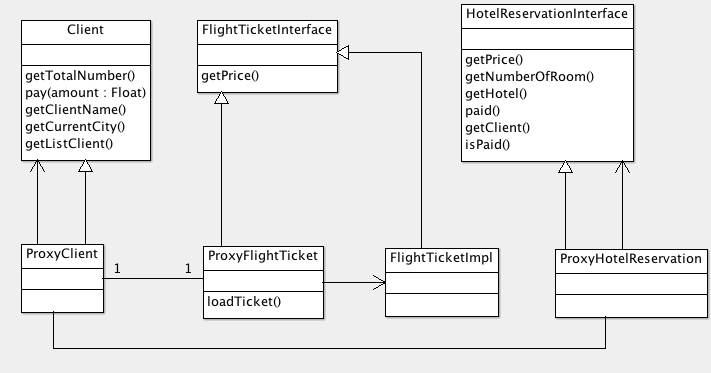
\includegraphics[width=12cm]{project/images/proxy.png}
\caption{Class diagram of proxies}
\end{figure}

\newpage
\subsection{Composite}
Composite pattern is used to describe a group of obejcts that could be treated almost as the same way as a single one. There are two composite in our program. 
\begin{itemize}
\item Client: as clients could booking the services as a group, a group of clients should be considered like one client. 
\item Travel with services: a travel package that consist of many trips to many cities, is still a travel.
\end{itemize}

\begin{figure}[h]
\centering
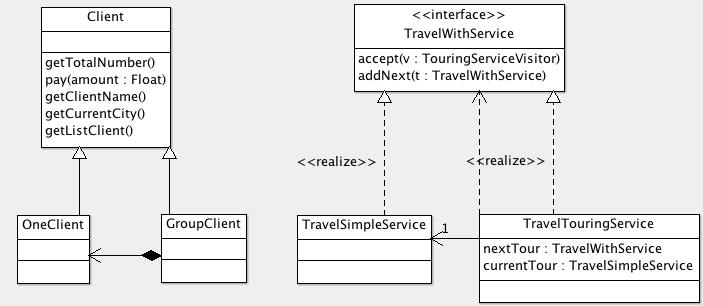
\includegraphics[width=12cm]{project/images/composite.png}
\caption{Class diagram of composite patterns}
\end{figure}

\paragraph{}
The implementation of composite pattern could be varied to adapt to the programer's intention. In this program's context, the \textit{GroupClient} consists of a list of \textit{OneClient}. In case of travel pattern, \textit{TravelTouringService}, a travel that go through many cities, use a recurrence relation that point to one other object of the same class.

\newpage
\subsection{Decorator}